% This is the Reed College LaTeX thesis template. Most of the work
% template. Later comments etc. by Ben Salzberg (BTS). Additional
% restructuring and APA support by Jess Youngberg (JY).
% Your comments and suggestions are more than welcome; please email
% them to cus@reed.edu
%
% See http://web.reed.edu/cis/help/latex.html for help. There are a
% great bunch of help pages there, with notes on
% getting started, bibtex, etc. Go there and read it if you're not
% already familiar with LaTeX.
%
% Any line that starts with a percent symbol is a comment.
% They won't show up in the document, and are useful for notes
% to yourself and explaining commands.
% Commenting also removes a line from the document;
% very handy for troubleshooting problems. -BTS

% As far as I know, this follows the requirements laid out in
% the 2002-2003 Senior Handbook. Ask a librarian to check the
% document before binding. -SN

%%
%% Preamble
%%
% \documentclass{<something>} must begin each LaTeX document
\documentclass[12pt,twoside]{reedthesis}
% Packages are extensions to the basic LaTeX functions. Whatever you
% want to typeset, there is probably a package out there for it.
% Chemistry (chemtex), screenplays, you name it.
% Check out CTAN to see: http://www.ctan.org/
%%
\usepackage{graphicx,latexsym}
\usepackage{amssymb,amsthm,amsmath}
\usepackage{longtable,booktabs,setspace}
\usepackage{chemarr} %% Useful for one reaction arrow, useless if you're not a chem major
\usepackage{rotating}

% Modified by CII
\usepackage[hyphens]{url}
\usepackage{hyperref}

% Added by CII (Thanks, Hadley!)
% Use ref for internal links
\renewcommand{\hyperref}[2][???]{\autoref{#1}}
\def\chapterautorefname{Chapter}
\def\sectionautorefname{Section}
\def\subsectionautorefname{Subsection}

\usepackage{caption}
\captionsetup{width=5in}

% \usepackage{times} % other fonts are available like times, bookman, charter, palatino

\title{Hierarchical Models for Crowdsourced Bicycle Route Ratings}
\author{Will Jones}
% The month and year that you submit your FINAL draft TO THE LIBRARY (May or December)
\date{May 2016}
\division{Mathematics and Natural Sciences}
\advisor{Andrew Bray}
%If you have two advisors for some reason, you can use the following
%\altadvisor{Your Other Advisor}
%%% Remember to use the correct department!
\department{Mathematics}
% if you're writing a thesis in an interdisciplinary major,
% uncomment the line below and change the text as appropriate.
% check the Senior Handbook if unsure.
%\thedivisionof{The Established Interdisciplinary Committee for}
% if you want the approval page to say "Approved for the Committee",
% uncomment the next line
%\approvedforthe{Committee}

% Below added by CII

\renewcommand{\contentsname}{Table of Contents}

\setlength{\parskip}{0pt}

\providecommand{\tightlist}{%
  \setlength{\itemsep}{0pt}\setlength{\parskip}{0pt}}

\Acknowledgements{
I want to thank a few people.
}

\Dedication{
You can have a dedication here if you wish.
}

\Preface{
This is an example of a thesis setup to use the reed thesis document
class.
}

\Abstract{
The preface pretty much says it all.
}


%%
%% End Preamble
%%
%

\begin{document}

      \maketitle
  
  \frontmatter % this stuff will be roman-numbered
  \pagestyle{empty} % this removes page numbers from the frontmatter

      \begin{acknowledgements}
      I want to thank a few people.
    \end{acknowledgements}
  
      \begin{preface}
      This is an example of a thesis setup to use the reed thesis document
      class.
    \end{preface}
  
  % Add table of abbreviations?

      \hypersetup{linkcolor=black}
    \setcounter{tocdepth}{2}
    \tableofcontents
  
      \listoftables
  
      \listoffigures
  
      \begin{abstract}
      The preface pretty much says it all.
    \end{abstract}
  
      \begin{dedication}
      You can have a dedication here if you wish.
    \end{dedication}
  
  \mainmatter % here the regular arabic numbering starts
  \pagestyle{fancyplain} % turns page numbering back on

  \chapter*{Introduction}\label{introduction}
  \addcontentsline{toc}{chapter}{Introduction}
  
  Knock Software's \emph{Ride Report} app combines a simple
  thumbs-up/thumbs-down rating system with GPS traces of bicycle rides to
  compile a crowdsourced data set of which routes are and are not
  stressful for urban bicyclists.
  
  The app that collects the data is simple: \emph{Ride Report}
  automatically detects when a user start riding their bike, records the
  GPS trace of the route, and then prompts the user at the end of the ride
  to give either a thumbs-up or thumbs-down rating. From this, they were
  able to create a crude ``stress map'' of Portland, OR, which simply
  shows the average ride rating of rides going through each discretized
  ride segment.
  
  The app privileges reducing barriers to response to increase sample size
  over ensuring quality and consistent responses. This presents the first
  problem: how can we analyze ratings when riders are likely rating rides
  inconsistently?
  
  At the same time, we have another challenge. We have ratings associated
  with routes, but we would like to know the effect of particular road
  segments, for both inference (what effect does this road segment have on
  the rating?) and prediction (given a route, what do we expect the rating
  to be?) purposes.
  
  \section{Accounting for Rider Rating
  Variance}\label{accounting-for-rider-rating-variance}
  
  For ratings we are interested in modeling variance between riders (as we
  might expect different rides to rate differently on average) and within
  riders (as riders may not rate the same route and conditions the same
  every time). To model this, we propose using multilevel regression, with
  random effects from each rider. This approach has been used in similar
  situations, in one case to model sexual attraction\footnote{Mackaronis,
    Strassberg, Cundiff, \& Cann (2013)}.
  
  In a multilevel model, we fit a regression where a slope of intercept
  term is a random variable whose distribution is unique to all the
  groupings. For example, if we let \(r_i\) be the rating of the \(i\)th
  ride, \(X_i\) be the ride-level variables, then we can fit a regression:
  
  \[\mathbb{P}(r_i = 1) = \text{logit}^{-1} 
  \left( \alpha_{j[i]} + \beta \cdot X_i \right) ,\] where \(\alpha_j\) is
  the contribution of the \(j\) rider:
  \[\alpha_j \sim N (\mu_\alpha, \sigma^2_j).\]
  
  We explore multilevel model further in Section 2.1 and multilevel models
  for riders in Section 4.2.
  
  \section{Addressing Road Segments as a
  Level}\label{addressing-road-segments-as-a-level}
  
  We examine multiple approaches to modeling road segments. In the first,
  we regard road segments as groups rides belong to, with the catch that
  rides can belong to multiple of these groups.
  
  \chapter{Data Sources}\label{rmd-basics}
  
  Here is a brief introduction into using \emph{R Markdown}.
  \emph{Markdown} is a simple formatting syntax for authoring HTML, PDF,
  and MS Word documents. \emph{R Markdown} provides the flexibility of
  \emph{Markdown} with the implementation of \textbf{R} input and output.
  For more details on using \emph{R Markdown} see
  \url{http://rmarkdown.rstudio.com}.
  
  Be careful with your spacing in \emph{Markdown} documents. While
  whitespace largely is ignored, it does at times give \emph{Markdown}
  signals as to how to proceed. As a habit, try to keep everything left
  aligned whenever possible, especially as you type a new paragraph. In
  other words, there is no need to indent basic text in the Rmd document
  (in fact, it might cause your text to do funny things if you do).
  
  \section{Ride Report}\label{ride-report}
  
  It's easy to create a list. It can be unordered like
  
  \begin{itemize}
  \itemsep1pt\parskip0pt\parsep0pt
  \item
    Item 1
  \item
    Item 2
  \end{itemize}
  
  or it can be ordered like
  
  \begin{enumerate}
  \def\labelenumi{\arabic{enumi}.}
  \itemsep1pt\parskip0pt\parsep0pt
  \item
    Item 1
  \item
    Item 2
  \end{enumerate}
  
  Notice that I intentionally mislabeled Item 2 as number 4.
  \emph{Markdown} automatically figures this out! You can put any numbers
  in the list and it will create the list. Check it out below.
  
  To create a sublist, just indent the values a bit (at least four spaces
  or a tab). (Here's one case where indentation is key!)
  
  \begin{enumerate}
  \def\labelenumi{\arabic{enumi}.}
  \itemsep1pt\parskip0pt\parsep0pt
  \item
    Item 1
  \item
    Item 2
  \item
    Item 3
  
    \begin{itemize}
    \itemsep1pt\parskip0pt\parsep0pt
    \item
      Item 3a
    \item
      Item 3b
    \end{itemize}
  \end{enumerate}
  
  \section{Weather Data}\label{weather-data}
  
  Make sure to add white space between lines if you'd like to start a new
  paragraph. Look at what happens below in the outputted document if you
  don't:
  
  Here is the first sentence. Here is another sentence. Here is the last
  sentence to end the paragraph. This should be a new paragraph.
  
  \emph{Now for the correct way:}
  
  Here is the first sentence. Here is another sentence. Here is the last
  sentence to end the paragraph.
  
  This should be a new paragraph.
  
  \section{Road Data}\label{road-data}
  
  When you click the \textbf{Knit} button above a document will be
  generated that includes both content as well as the output of any
  embedded \textbf{R} code chunks within the document. You can embed an
  \textbf{R} code chunk like this (\texttt{cars} is a built-in \textbf{R}
  dataset):
  
  \chapter{Data Transformation}\label{data-trans}
  
  \section{Working in Road Networks}\label{working-in-road-networks}
  
  \section{Using Nearest Neighbor Search for Map Matching
  Data}\label{using-nearest-neighbor-search-for-map-matching-data}
  
  \section{Missing Data}\label{missing-data}
  
  \chapter{Methods}\label{methods}
  
  As an undergraduate thesis, a lot of research into methodology was done.
  Here I go through some of the essential methodology, while establishing
  the notation I will use for the rest of this paper.
  
  \section{Logistic Regression}\label{logistic-regression}
  
  With logistic regression, we seek to fit a model where the response
  variable is binary. We might consider the response variable, \(Y\), a
  Bernoulli random variable,
  
  \[Y = \text{Bernoulli}(p),\]
  
  where \(p\) is the probability that an observation \(y_i = 1,\) for any
  \(i\). (As a binary variable, the support of \(Y\) is \(\{0,1\}\), so
  \(y_i = 0\) otherwise.) Thus, in predicting and making inference about a
  Bernoulli variable, we are concerned with \(p\) and how it varies with
  respect to other quantities.
  
  Logistic regression is, as we will see, one form of regression
  generalized from linear regression.
  
  Linear regression is the first form of regression most people learn:
  find the line
  
  \[y_i = \beta_0 + \beta_1 x_1 + \ldots + \beta_j x_j + \epsilon,\]
  
  based on data with response variable \(y_i\) and \(j\) predictor
  variables \(x_i\), coefficients \(\beta_0, \ldots, \beta_j\), and error
  term \(\epsilon \sim N(0, \sigma^2)\). We can equivalently write,
  
  \[Y \sim N(\beta_0 + \beta_1 x_1 + \ldots + \beta_j x_j, \sigma^2).\]
  
  Generalized linear regression uses a ``link function,'' \(g\), to modify
  the regression:
  
  \[g(y_i) = \beta_0 + \beta_1 x_1 + \ldots + \beta_j x_j + \epsilon.\]
  
  Logistic regression is a form of generalized regression where the `link'
  function is the logit function, \(\text{logit}:[0,1] \to \mathbb{R}\):
  
  \[ \text{logit} (p) = \log \left(\frac{p}{1-p}\right), \]
  
  also known as the log-odds, odds being \(p/1-p\) for any probability
  \(p\). So we can model this as a Bernoulli random variable where the
  probability of a 1 is:
  
  \[\mathbb{P} (y_i = 1) = \text{logit}^{-1} (\beta_0 + \beta_1 x_1 + \ldots + \beta_j x_j).\]
  
  Notice that the inverse logit function maps values from \(\mathbb{R}\)
  to \([0,1]\). The function provides a convenient way to map linear
  combinations of other variables onto values that are valid
  probabilities. Other such functions exist and are also used for
  regression of binary variables, such as the probit function.
  
  \begin{center}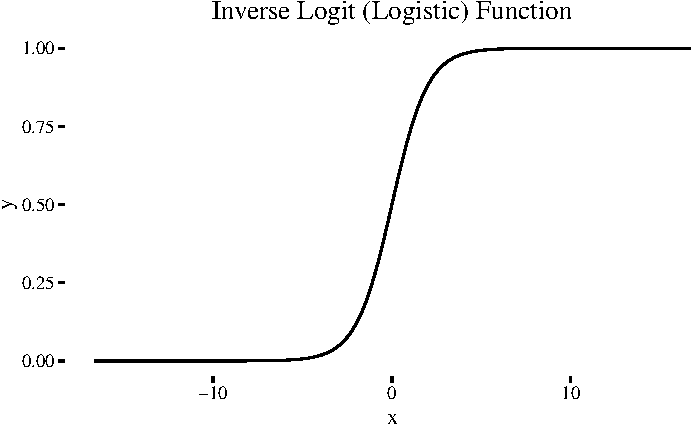
\includegraphics{thesis_files/figure-latex/unnamed-chunk-1-1} \end{center}
  
  \section{Hierarchical Models and Mixed Effects
  Models}\label{hierarchical-models-and-mixed-effects-models}
  
  Many data sets contain nested structures when viewed in some way. For
  example, a data set of student test scores may contain information about
  the schools and districts they are in. Or a dataset of soil samples may
  have multiple samples from each of a set of different sites. In the
  dataset we examine, rides can be grouped by rider.
  
  Mutlilevel models allow us to address these kinds of relationships in
  regression models. They provide a number of computational advantages, as
  we shall describe later.
  
  \subsection{Description and Notation}\label{description-and-notation}
  
  These models of course work for other forms of regression, but we will
  focus on logistic regression, as it is the method we use in this paper.
  We will be using notation adapted from Gelman's description of
  multilevel models. Consider a data set composed of
  
  \begin{itemize}
  \itemsep1pt\parskip0pt\parsep0pt
  \item
    \(i\) observations of a binary response variable \(y_i\),
  \item
    \(m\) observation level predictors \(X_i = x_i^1, \ldots, x_i^m\),
  \item
    \(j\) groups in which the observations are split into,
  \item
    \(l\) group level predictors
    \(U_{j[i]} = u_{j[i]}^1, \ldots, u_{j[i]}^l\), where \(j[i]\) is the
    group of the \(i\)th observation,.
  \end{itemize}
  
  We could fit a model where the intercept varies by group:
  
  \[\mathbb{P} (y_i = 1) = \text{logit}^{-1}
  (\alpha_{j[i]} + X_i \beta),\]
  \[\alpha_{j[i]} \sim N(\gamma_0 + U_{j[i]} \gamma, \sigma_{\alpha}^2),\]
  
  where \(\alpha_{j[i]}\) is the intercept for the \(j\)th group,
  \(\beta\) are the coefficients for the observation-level predictors,
  \(\gamma_0\) are the group-level intercepts, and \(\gamma\) are the
  coefficients for the group-level predictors. We could also imagine a
  similar model where there are no group level predictors, such that we
  simply have different intercepts for each group,
  \[\alpha_{j[i]} \sim N(\gamma_0, \sigma_{\alpha}^2),\]
  
  We can also consider a model that has slopes varying by group. For
  simplicity, let's consider just one observation level predictor,
  \(x_i\), that will have varying slopes \(\beta_{j[i]}\) as well as one
  group level predictor. We could specify the model as,
  
  \[\mathbb{P} (y_i = 1) = \text{logit}^{-1}
  (\alpha_{j[i]} + \beta_{j[i]} x_i),\]
  
  \[
  \left(
  \begin{array}{c}
  \alpha_{j}\\
  \beta_{j}
  \end{array}
  \right) =
  N \left(
  \left(
  \begin{array}{c}
  \gamma_0^\alpha + \gamma_1^\alpha u_j\\
  \gamma_0^\beta + \gamma_1^\beta u_j
  \end{array}
  \right),
  \left(
  \begin{array}{cc}
  \sigma^2_\alpha & \rho \sigma_\alpha \sigma_\beta\\
  \rho \sigma_\alpha \sigma_\beta & \sigma^2_\beta
  \end{array}
  \right)
  \right).
  \]
  
  \subsection{Examples and Advantages}\label{examples-and-advantages}
  
  Gelman puts forward a framework for thinking about multilevel models as
  a comprimise between no-pooling and complete pooling. For example, for
  the school example, one could fit a classical regression ignoring the
  schoolwide data, with students as the level of observation. (That would
  be ``no pooling''.) Alternatively, one could fit a separate regression
  for each school.
  
  \chapter{Model 1: Rides and Riders}\label{model-1-rides-and-riders}
  
  We start out model simply and then building up. The first problem to
  approach is handling rider variance. This sections describes how we do
  that using a random effects terms and demonstrates the improvement in
  the models fit and predictive accuracy over more classical models.
  
  \section{Choosing Ride-Level
  Parameters}\label{choosing-ride-level-parameters}
  
  \section{Adding Random Effects from
  Riders}\label{adding-random-effects-from-riders}
  
  \section{Evaluating the Ride-Level
  Models}\label{evaluating-the-ride-level-models}
  
  \chapter{Model 2: Segments as a New
  Level}\label{model-2-segments-as-a-new-level}
  
  \section{Choosing Segment-Level
  Parameters}\label{choosing-segment-level-parameters}
  
  \section{Evaluating Segment-Level
  Models}\label{evaluating-segment-level-models}
  
  \chapter{Model 3: A Spatial Model}\label{model-3-a-spatial-model}
  
  \chapter{Comparative Evaluation}\label{comparative-evaluation}
  
  \chapter*{Conclusion}\label{conclusion}
  \addcontentsline{toc}{chapter}{Conclusion}
  
  \setcounter{chapter}{4} \setcounter{section}{0}
  
  If we don't want Conclusion to have a chapter number next to it, we can
  add the \texttt{\{.unnumbered\}} attribute. This has an unintended
  consequence of the sections being labeled as 3.6 for example though
  instead of 4.1. The \LaTeX~commands immediately following the Conclusion
  declaration get things back on track.
  
  \subsubsection{More info}\label{more-info}
  
  And here's some other random info: the first paragraph after a chapter
  title or section head \emph{shouldn't be} indented, because indents are
  to tell the reader that you're starting a new paragraph. Since that's
  obvious after a chapter or section title, proper typesetting doesn't add
  an indent there.
  
  \backmatter
  
  \chapter{References}\label{references}
  
  \noindent
  
  \setlength{\parindent}{-0.20in} \setlength{\leftskip}{0.20in}
  \setlength{\parskip}{8pt}
  
  Cressie, N., \& Wikle, C. K. (2011). \emph{Statistics for
  spatio-temporal data}. John Wiley \& Sons.
  
  Gelman, A., \& Hill, J. (2006). \emph{Data analysis using regression and
  multilevel/Hierarchical models}. The Edinburgh Building, Cambridge CB2
  8RU, UK: Cambridge University Press, New York.
  
  Mackaronis, J. E., Strassberg, D. S., Cundiff, J. M., \& Cann, D. J.
  (2013). Beholder and beheld: A multilevel model of perceived sexual
  appeal. \emph{Archives of Sexual Behavior}.


  % Index?

\end{document}

